\documentclass[12pt,a4paper,onecolumn]{article}
\usepackage[utf8]{inputenc}
\usepackage[spanish, es-tabla]{babel}
\usepackage{amsmath}
\usepackage{amsfonts}
\usepackage{amssymb}
\usepackage{graphicx}
\usepackage[version=4]{mhchem}
\usepackage[left=2.5cm,right=2.5cm,top=2.5cm,bottom=2.5cm]{geometry}
\usepackage{cite}
\usepackage{float}
\usepackage{hyperref}
\usepackage[font=small,labelfont=bf]{caption} % Pone en negrita Figura X y reduce el tamaño de la descripción de un gráfico
\author{Jessica Katherine Gaona Alvarado}
\title{Simulación PET con \ce{^{11}C}, \ce{^{13}N}, \ce{^{15}O}, \ce{^{18}F}, \ce{^{82}Rb} y \ce{^{68}Ga}}

\begin{document}
\maketitle
\date
\begin{abstract}
	La simulación por emisión de positrones nos permite analizar \ldots
	
	Este trabajo completo conjuntamente con todos los archivos que utiliza el documento .tex lo podemos encontrar en un repositorio que ha sido creado para tal efecto y su enlace es el siguiente \url{https://github.com/JessicaGaonaA/proyecto_final.git}. Este documento .tex contiene a lo largo del artículo todos los aspectos que recomienda el profesor del curso para la elaboración del artículo: título, resumen, palabras clave, introducción, estado del arte, imágenes y tablas, fórmulas y bibliografía.
	
\end{abstract}


\section{Introducción}
En la presente práctica usaremos el código de simulación Monte Carlo PENELOPE para estudiar dos aspectos relacionados con el PET. En primera instancia se estudiará la distribución de posiciones de aniquilación de los positrones emitidos considerando un espectro continuo, y en segunda instancia se considera una fuente monoenergética con energía igual a la energía máxima del espectro para diferentes radionúclidos emisores $\beta^+$ (\ce{^{11}C}, \ce{^{13}N}, \ce{^{15}O}, \ce{^{18}F}, \ce{^{82}Rb} y \ce{^{68}Ga}). Se hará un segundo estudio considerando una geometría esférica ideal que simula la cabeza de un paciente donde se analizará el espectro de los fotones que llegan al detector como consecuencia de aniquilación de los positrones. Para ambos estudios se utilizará los radionúclidos que constan en la tabla \ref{radio}, y en el segundo estudio además se variará la geometría para observar sus efectos en la superficie detectora.

\section{Tomografía por emisión de positrones (PET)}
Es una técnica diagnóstica de medicina  nuclear que se basa en la detección de los rayos gamma de 511 keV que se generan en la aniquilación de los positrones que emite un determinado radiofármaco inyectado previamente a un paciente. Una vez inyectado el radiofármaco al paciente, se sitúa éste en un detector de rayos gamma con una electrónica que permite realizar análisis de coincidencias.
\begin{equation}
DBE=-\frac{\log S}{\alpha}=nd\Big(1+\frac{d}{\alpha/\beta}\Big)
\end{equation}
\begin{figure}[h]
	\centering
	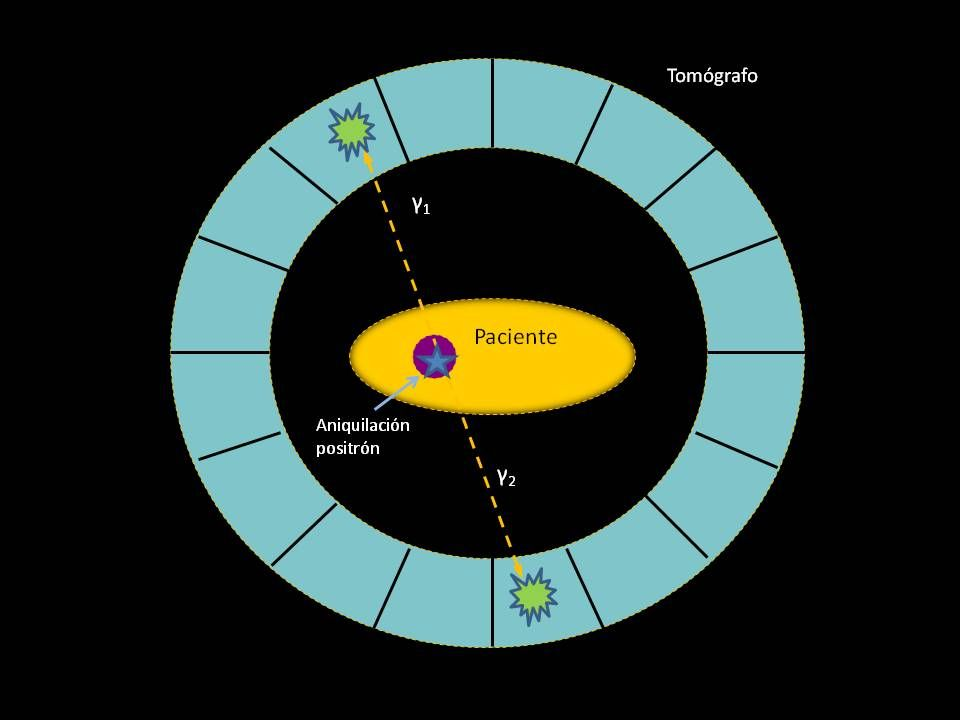
\includegraphics[width=0.5\linewidth]{aniquila}
	\caption{Esquema de detección de un par de fotones en coincidencia.}
	\label{fig:aniquila}
\end{figure}

Los positrones  emitidos recorrerán una pequeña distancia y se aniquilarán con algún electrón del medio produciendo dos fotones de 511 keV colineales como se observa en la figura \ref{fig:aniquila}.
\section{Radionúclidos emisores $\beta^+$}
La tomografía por emisión de positrones requiere biomoléculas marcadas con isótopos emisores de positrones. Estos radionúclidos son isótopos inestables con un exceso de protones que tienden a la estabilidad transformando protones en neutrones, conviertiéndose en otro elemento de vida media corta. El \ce{^{18}F} es uno de los varios isótopos del flúor que se utilizan habitualmente en el radiomarcado de biomoléculas para la PET debido a su capacidad de emisión de positrones y semivida de 109.8 min \cite{alauddin2012}. El radiofármaco más comúnmente usado es el flúordeoxiglucosa (\ce{FDG}) para la detección temprana de tumores malignos, gracias al mayor índice glicolítico que poseen las células neoplásicas \cite{carranza2005}.

Entre los radionúclidos convencionales constan el \ce{^{11}C}, \ce{^{13}N}, \ce{^{15}O}, \ce{^{18}F}, y los añadidos en los últimos 12 años \ce{^{82}Rb} y \ce{^{68}Ga}. En la tabla \ref{radio} se observa el tiempo de semivida, energía máxima y alcance en agua de cada uno de los radionúclidos mencionados.

\begin{table} [H]
	\begin{center}
		\begin{tabular}{c c c c} 
			\hline 
			Emisor	& \ce{T_{1/2} (min)} & \ce{E_{max} (MeV)} & Alcance (mm) \\ 
			\hline 
			\ce{^{11}C}	& 20.3 & 0.97 & 3.67 \\ 
			
			\ce{^{13}N}	& 9.96 & 1.19 & 4.88 \\ 
			
			\ce{^{15}O}	& 2.07 & 1.70 & 7.92 \\ 
			
			\ce{^{18}F}	& 109.8 & 0.635 & 2.16 \\ 
			
			\ce{^{82}Rb} & 1.27 & 3.35 & 16.5 \\ 
			
			\ce{^{68}Ga} & 68.3 & 1.88 & 9.06 \\ 
			\hline 
			
		\end{tabular}
		\caption{Radionúclidos en PET}
		\label{radio} 
	\end{center}
\end{table}

\section{Materiales y Métodos}
\subsubsection*{Código PENELOPE}
Se usó el código de simulación Monte Carlo PENELOPE para estudiar dos aspectos relacionados con el PET (programa PET-1 y PET-2) que se explican más adelante. El código PENELOPE es un paquete de subrutinas escrito en Fortran 77. La complejidad de la interacción radiación-materia para una geometría y material arbitrarios implica que tengamos que utilizar técnicas numéricas ya que no se puede describir analíticamente el transporte de partículas en un medio. \cite{salvat2006}

\subsection*{Método}
Para la simulación se trabajó con el programa PET, PET-1 y PET-2, en el primero se consideró un espectro continuo de las posiciones de aniquilación de positrones en agua para radionúclidos emisores $\beta^+$ (\ce{^{11}C}, \ce{^{13}N}, \ce{^{15}O}, \ce{^{18}F}, \ce{^{82}Rb} y \ce{^{68}Ga}), la energía correspondiente a cada radioisótopo se obtiene de la tabla \ref{radio}. Además, se comparó el resultado con el obtenido para una fuente monoenergética con energía igual a la energía máxima del espectro para los diferentes radionúclidos. Para su comparación se presenta los resultados de la energía media en función de la posición mediante un ajuste de curvas.
  
Se realizó un segundo estudio considerando una geometría esférica ideal que simula la cabeza de un paciente donde se analizará el espectro de los fotones que llegan al detector como consecuencia de la aniquilación electrón-positrón. Se considera una esfera de 9 cm de agua simulando el cerebro, concéntrica a ella a 0.5 cm de la misma, situamos una corona esférica para simular el cráneo (hueso), el resto hasta los 45 cm corresponde a aire, y a partir de ahí se sitúa el detector (Pb). Para ambos estudios se utilizará los radionúclidos que constan en la tabla \ref{radio}, y en el segundo estudio además se variará la geometría para observar sus efectos en la superficie detectora. La información a analizar en ambos programas se obtiene de los histogramas generados (pos.his y ene.his).

\subsubsection*{Creación de materiales (.mat)}
La definición de agua, aire, hueso y plomo con extensión \textbf{.mat} que constan dentro del archivo de entrada tanto en PET-1 como en PET-2 se realizó en la carpeta pendbase con el ejecutable material.exe, en donde se puede generar material de dos formas: ingresando los datos de la composición desde el teclado o leyendo desde el archivo pdcompos.pen. En este trabajo se utilizó la segunda opción.

\subsubsection*{Definición del archivo (.in)}
En la definición del archivo de entrada constan los parámetros que dirigen nuestra simulación, entre ellos tenemos los materiales a interaccionar con la radiación, la energía máxima, número másico y atómico del elemento al que decae el radionúclido por emisión \ce{\beta^+}, y de acuerdo al programa para la extensión del histograma se considera la energía máxima del radionúclido y su alcance en el material usado, además en PET-2 se añade el radio de cada una de las superficies de la esfera. Todos los datos sobre los radionúclidos pueden cosultarse en la tabla \ref{radio}.

\section{Resultados y Discusión}
\subsection*{PET-1}
Tras la simulación en el espectro continuo se observa la distribución de posiciones de aniquilación electrón-positrón, mecanismo que se produce cuando los positrones emitidos por los radionúclidos interaccionan con un electrón en su camino dando origen a dos fotones que se desplazan colinealmente. En la figura \ref{fig:contrasteposfluor} se observa esta distribución donde el alcance de los positrones depende del alcance del radioisótopo usado. En la primera simulación para el caso  \ce{^{18}F} se ve que existe un alcance hasta aproximadamente 2.1 mm, y en el caso de la fuente monoenergética la distribución de posiciones se presenta desplazada hacia la izquierda con un máximo en 0.5 mm y un rango de [0, 0.7] mm.

En el primer caso con el mismo radionúclido se visualiza un espectro energético continuo de los positrones emitidos, Figura 3, con un máximo en 203 keV. Al usar una fuente monoenergética en el espectro energético se visualiza un único pico en 252 keV, Figura 4. El máximo en el espectro continuo y usando la fuente monoenergética varía de acuerdo a la energía máxima de cada radioisótopo.
\begin{figure}[h]
	\centering
	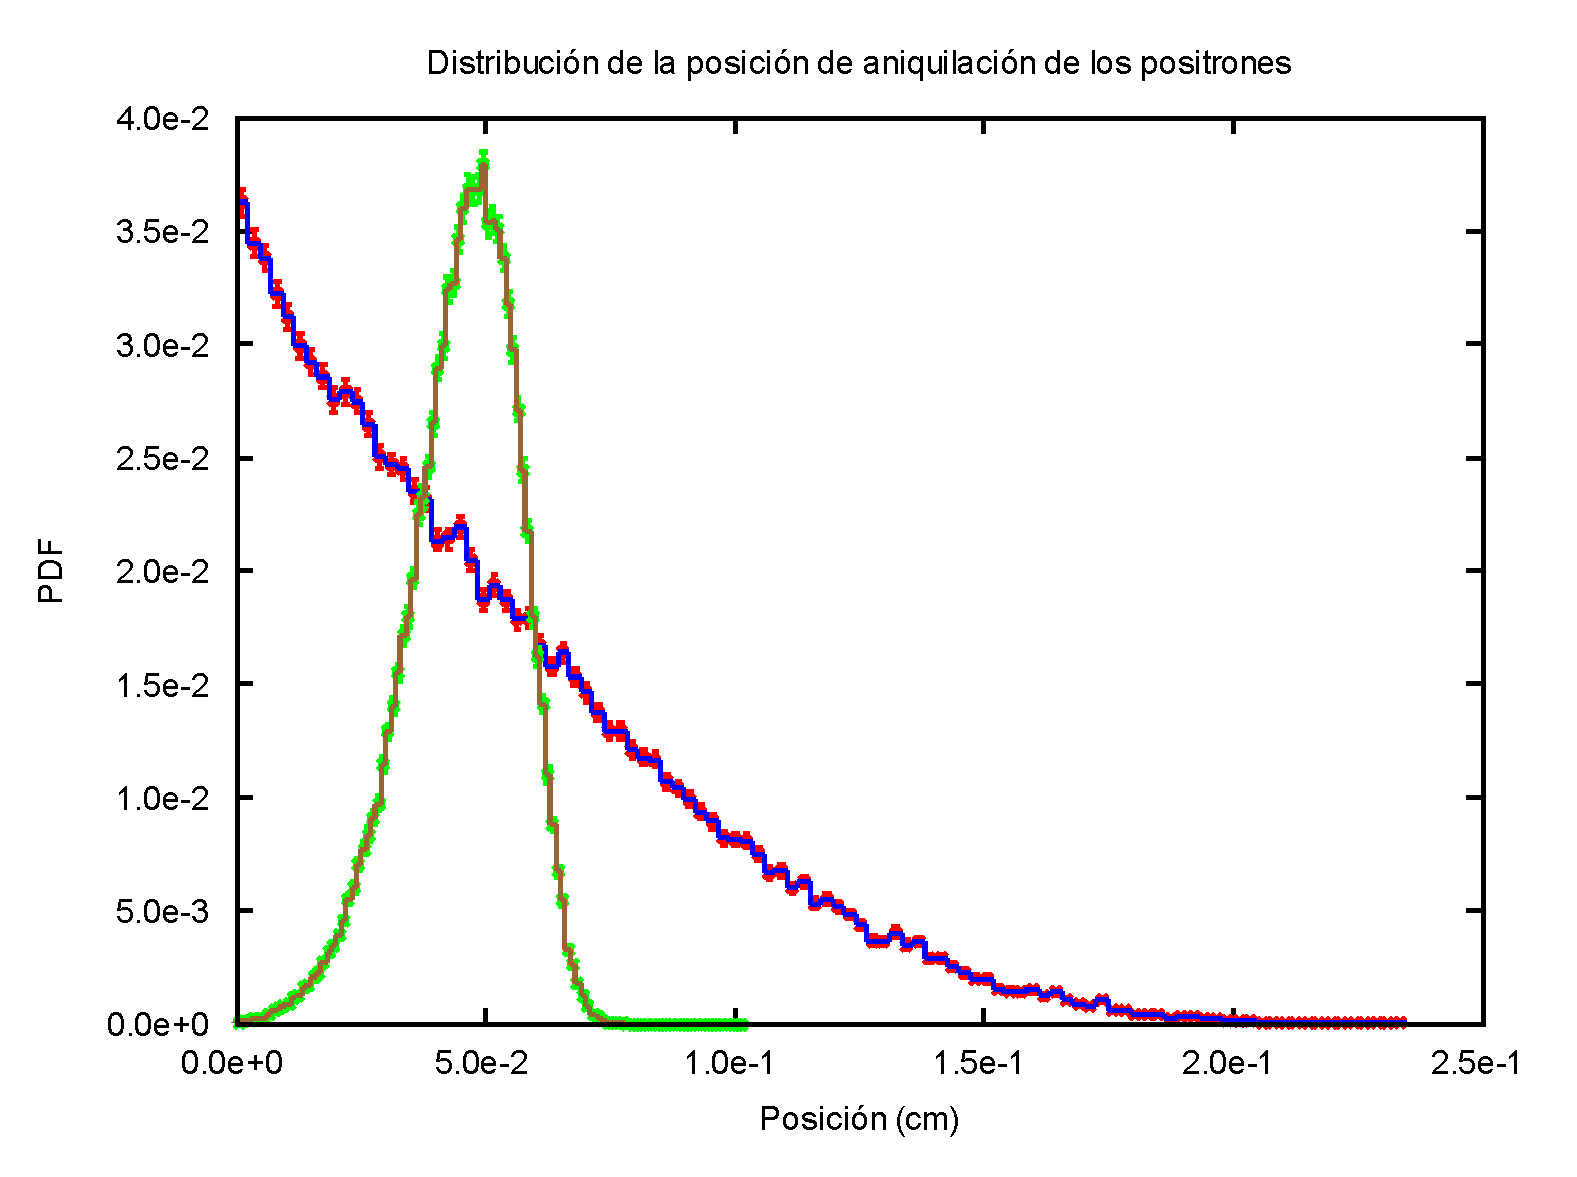
\includegraphics[width=0.7\linewidth]{../proyecto_final/contrasteposfluor}
	\caption{Posiciones de aniquilación de los positrones emitidos por el \ce{^{18}F}.}
	\label{fig:contrasteposfluor}
\end{figure}

\begin{figure}[H]
\centering
  \begin{minipage}{0.45\textwidth}
	\centering
    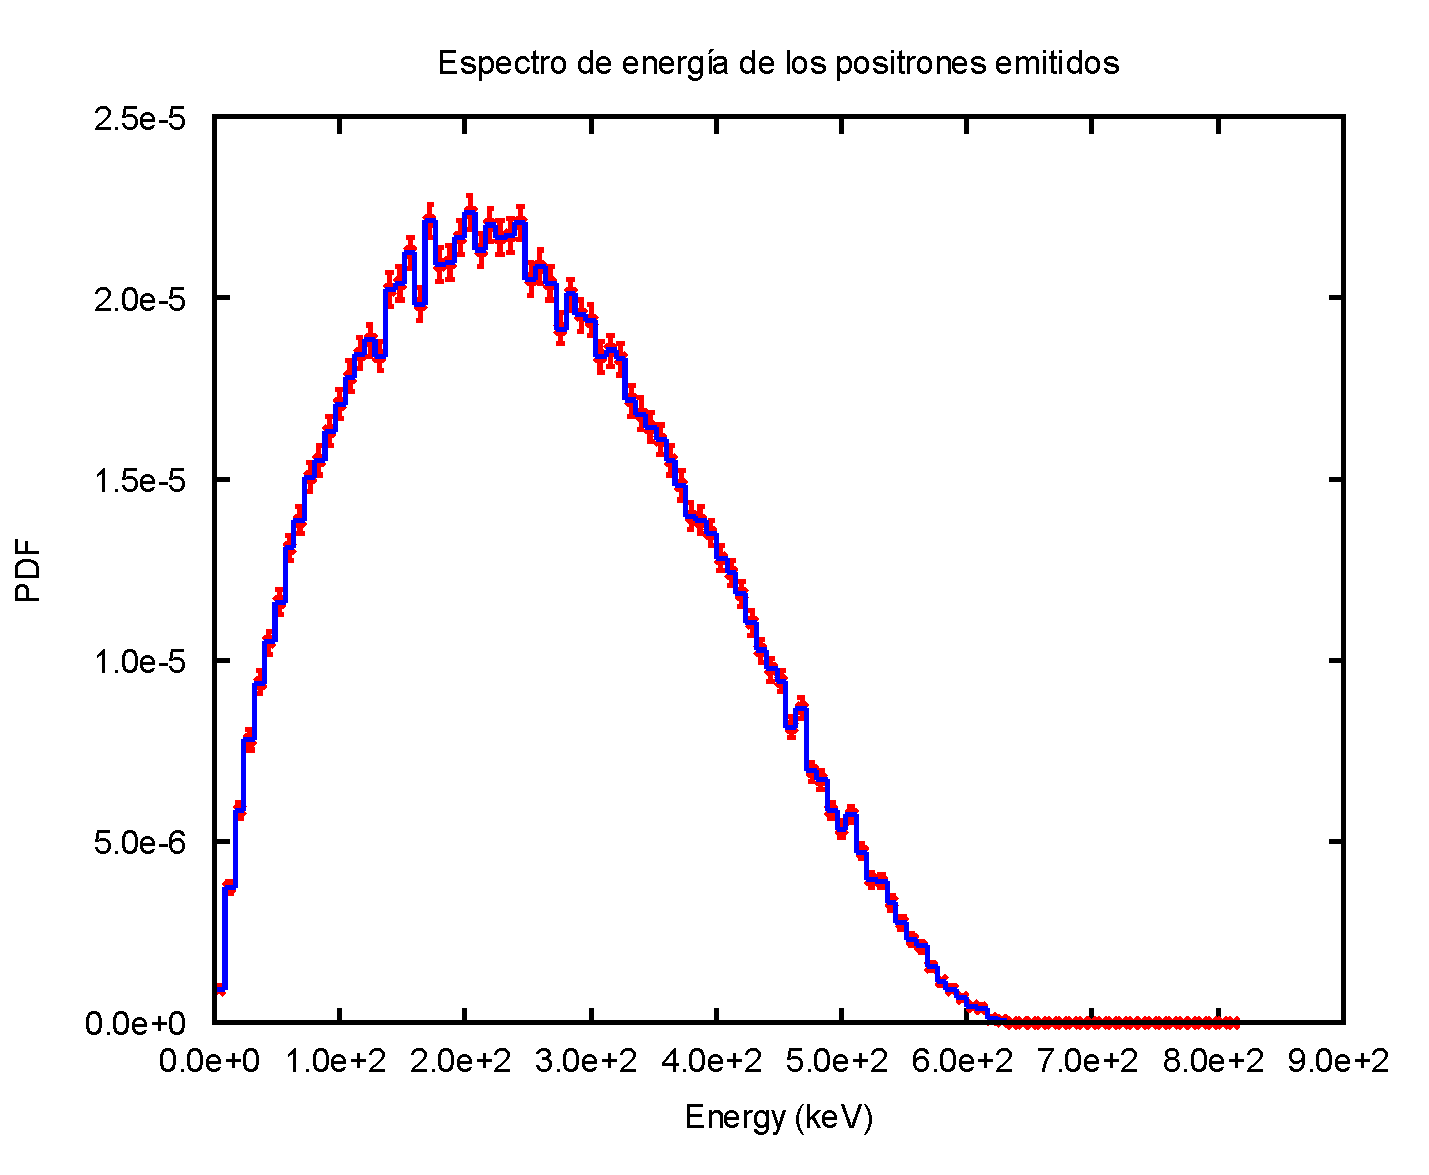
\includegraphics[scale=0.32]{../proyecto_final/1fluorcontene}
    \caption{Espectro continuo de energía del \ce{^{18}F}}
    \label{EspC1}
  \end{minipage}
  \hspace{2mm}
  \begin{minipage}{0.45\textwidth}
	\centering
	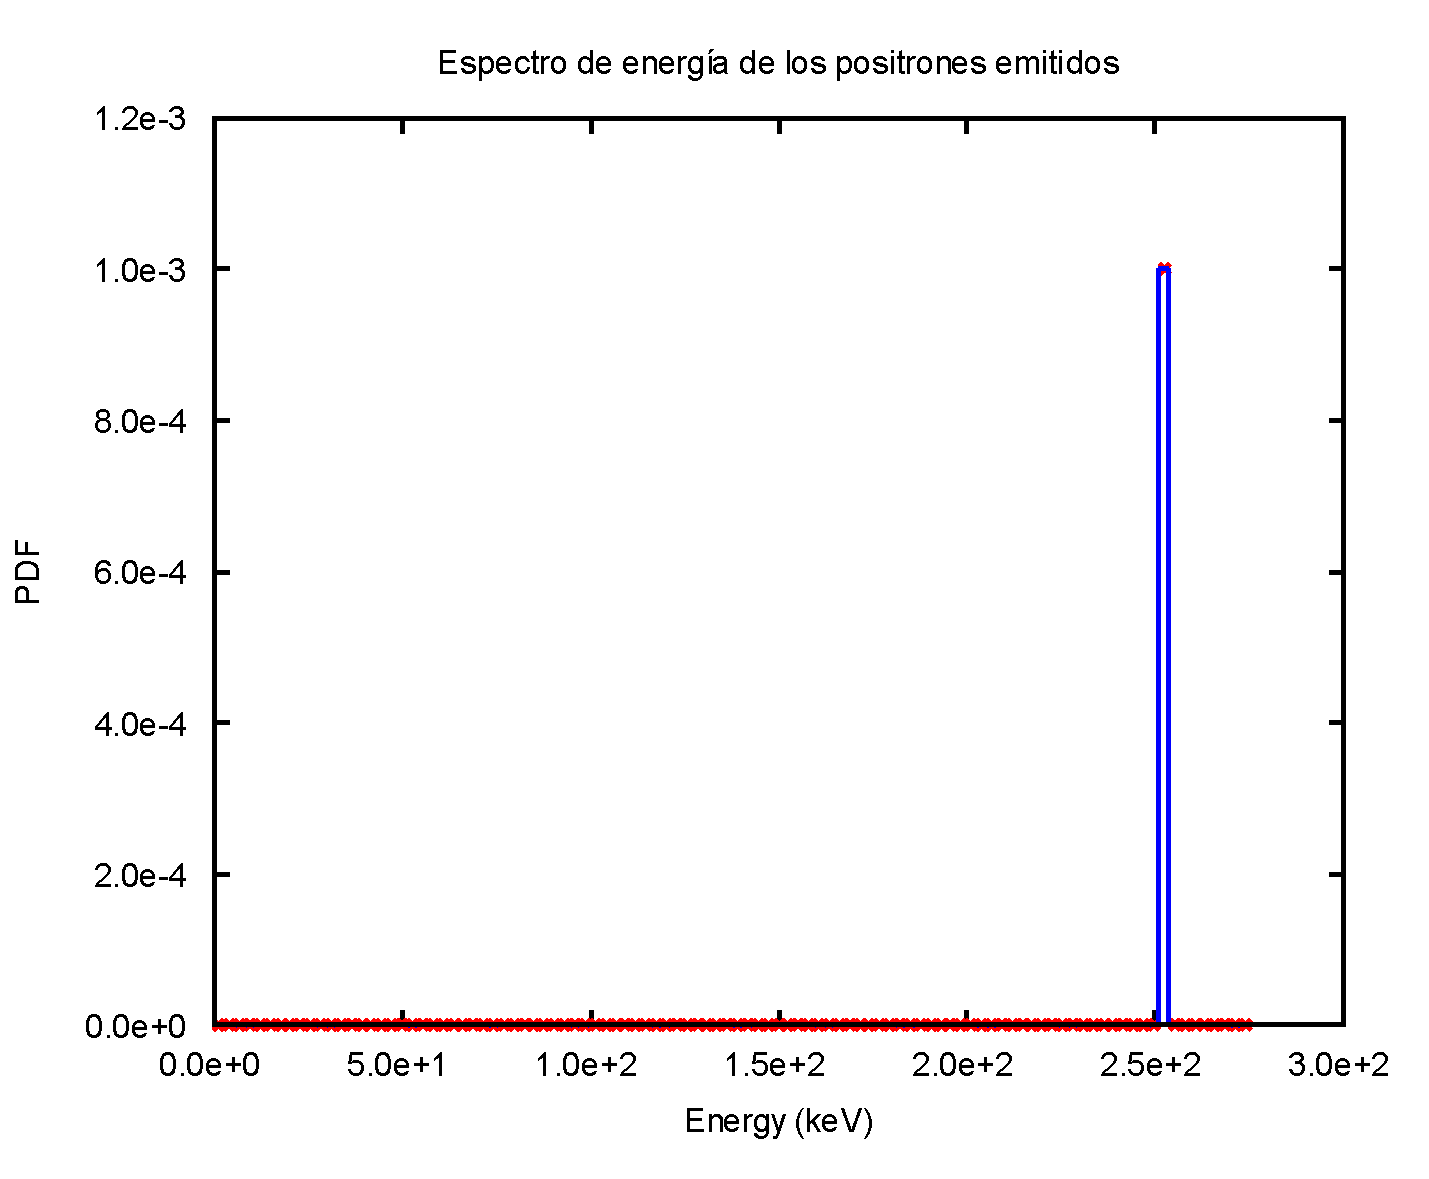
\includegraphics[scale=0.32]{../proyecto_final/1fluormonene}
	\caption{Espectro de energía de una fuente monoenergética de \ce{^{18}F}.}
	\label{fig:1fluormonene}
  \end{minipage}	
\end{figure}
El espectro energético y la distribución de posiciones de aniquilación de los positrones varía de acuerdo a la energía máxima y alcance de cada radionúclido. En el primer caso en la figura \ref{EspC1} se visualiza un espectro energético continuo, mientras que al usar una fuente monoenergética únicamente se visualiza un pico, figura \ref{fig:1fluormonene}. La distribución de posiciones de aniquilación al usar la fuente monoenergética se muestra desplazada hacia la izquierda. Ésto se puede apreciar mejor usando un ajuste de curvas, figura \ref{fig:eneposmedia}, donde consta la energía media en función de la posición de aniquilición de cada uno de los radionúclidos considerados en este trabajo. 
\begin{figure}[h]
	\centering
	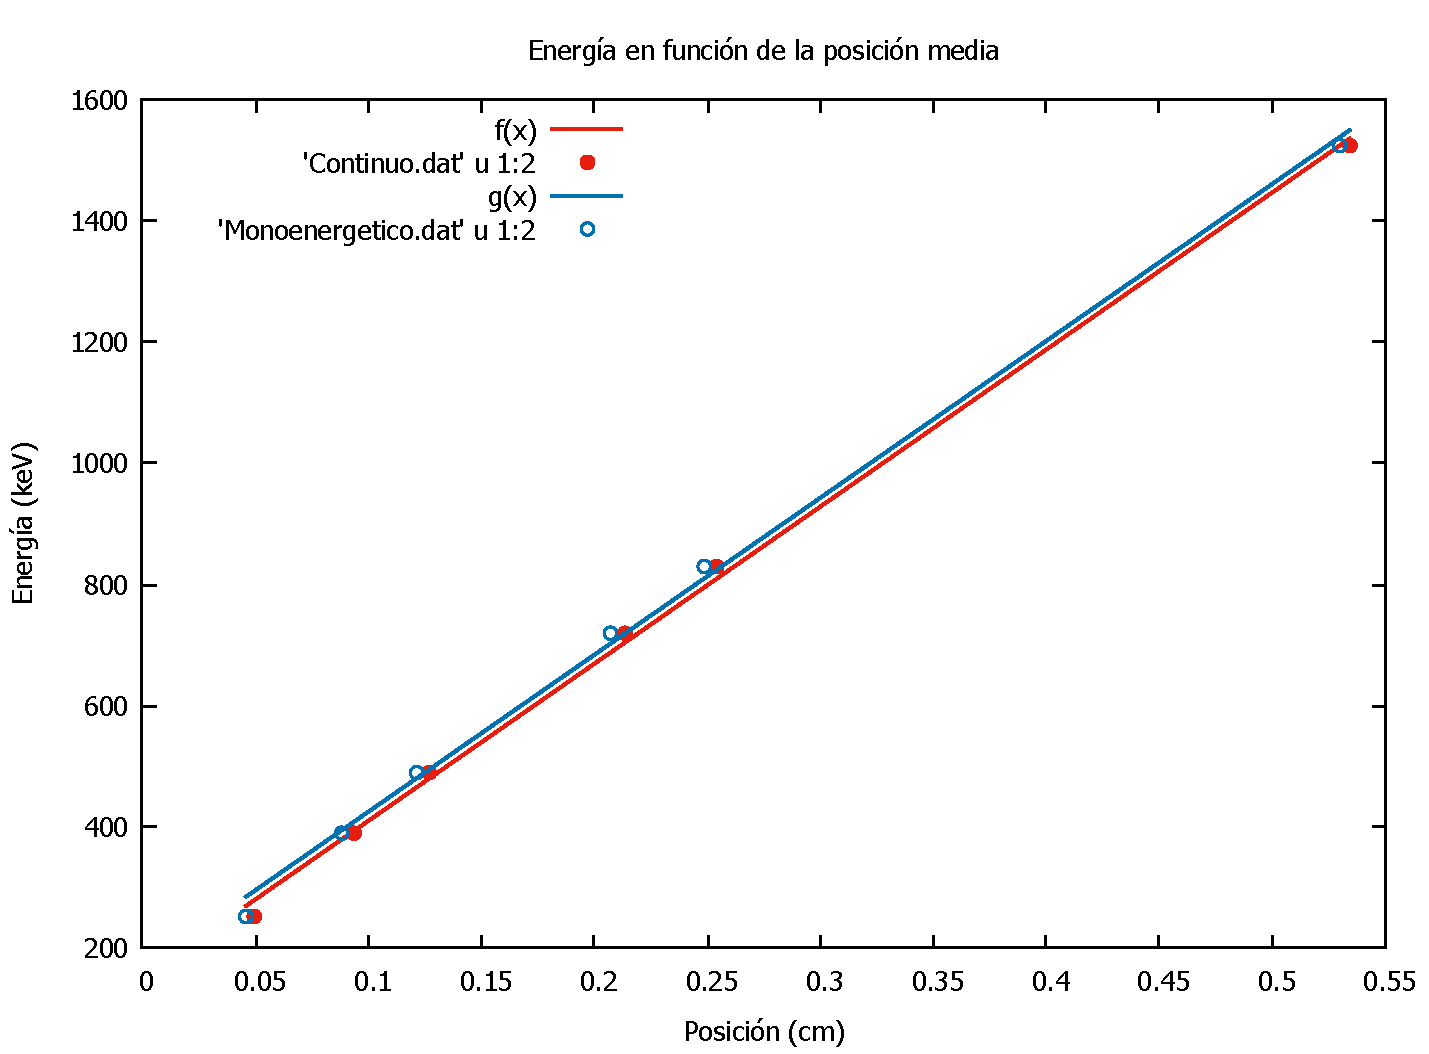
\includegraphics[width=0.7\linewidth]{../proyecto_final/ene_pos_media}
	\caption{Energía media en función de la posición de aniquilación de los positrones emitidos por el \ce{^{11}C}, \ce{^{13}N}, \ce{^{15}O}, \ce{^{18}F}, \ce{^{82}Rb} y \ce{^{68}Ga}.}
	\label{fig:eneposmedia}
\end{figure}
\subsection*{PET-2} 
Realizada la simulación se puede observar el espectro de fotones que llegan al detector como consecuencia de la aniquilación de los positrones emitidos por los radionúclidos considerados (emisores $\beta^+$). En la figura \ref{fig:fotonesdetectados} se observa el máximo de la función densidad de probabilidad para cada uno de los radioisótopos, ubicándose el \ce{^{18}F} con el máximo de la PDF entre ellos seguido por el \ce{^{11}C}, \ce{^{13}N}, \ce{^{15}O} y los radioisótopos añadidos en los últimos 12 años emisosores de positrones no biológicos \ce{^{68}Ga} y \ce{^{82}Rb}. El \ce{^{18}F} es bastante usado puesto que no hay un hidrógeno emisor de positrones. Ello hace que cualquier molécula del organismo pueda ser, en teoría, marcada con un isótopo radiactivo y utilizada para evidenciar un hecho bioquímico-molecular \cite{sanchez2006}. 

Si consideramos la cabeza del paciente de r = 9 cm con 0.25 y 0.5 cm de hueso un mayor número de fotones llegan al detector a 0.25 cm de hueso, figura \ref{fig:02505hueso}. En la figura \ref{fig:2sinhueso05cmhueso} se muestra la cabeza de un paciente con el mismo radio, con corona esférica de 0.5 cm y sin corona esférica. Se observa que cuando no hay la presencia de hueso el número de fotones detectados es mayor que cuando sí se considera los 0.5 cm de hueso, es decir con hueso hay una pequeña atenuación de los fotones registrada al llegar al detector. Esta atenuación también se pudo observar en la figura \ref{fig:02505hueso} con los 0.5 cm de hueso en comparación a los 0.25~cm.

Ahora simplemente añado texto falso Ahora simplemente añado texto falso Ahora simplemente añado texto falso Ahora simplemente añado texto falso Ahora simplemente.

\begin{figure}[h]
	\centering
	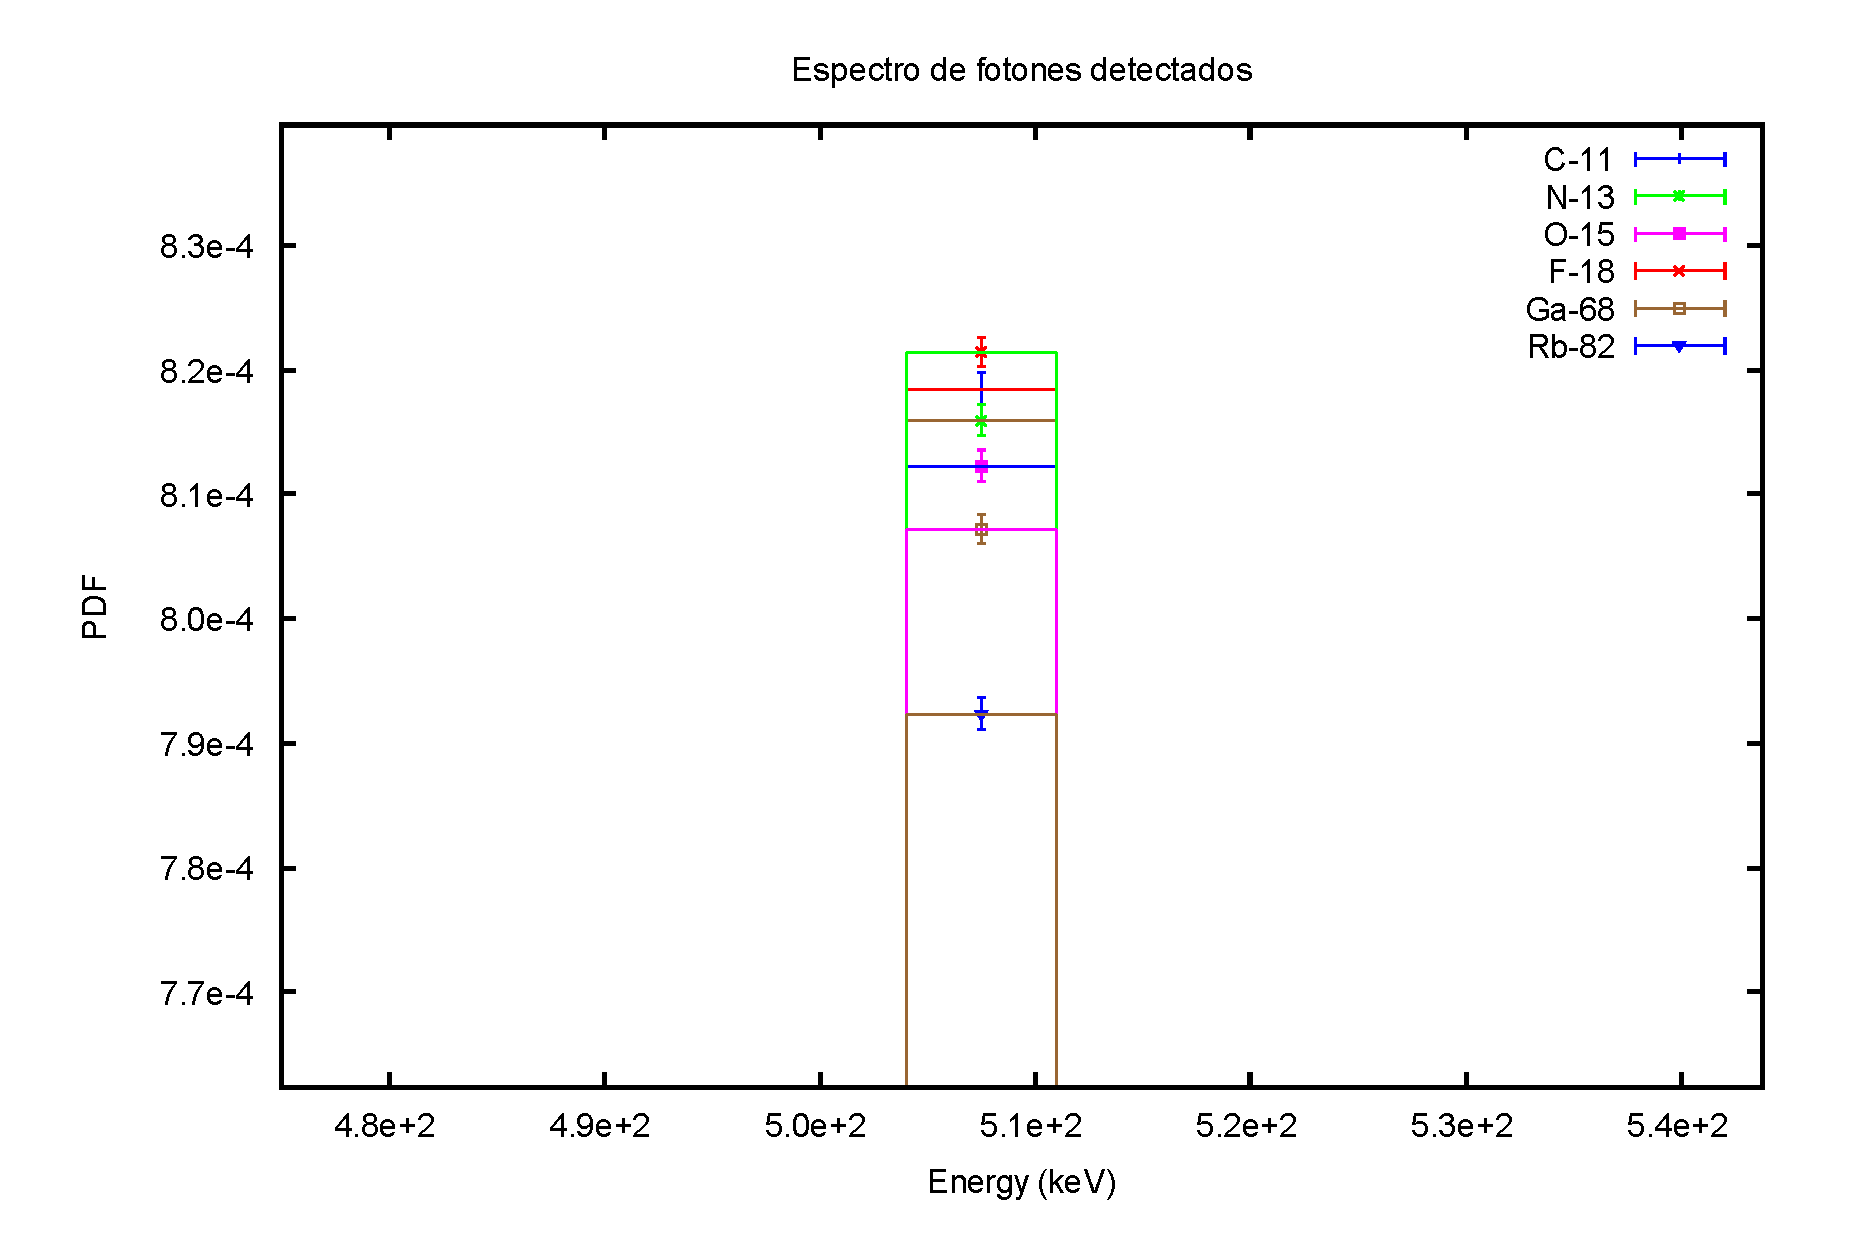
\includegraphics[width=0.7\linewidth]{../proyecto_final/fotonesdetectados}
	\caption{Espectro de fotones detectados de \ce{^{11}C}, \ce{^{13}N}, \ce{^{15}O}, \ce{^{18}F} y \ce{^{82}Rb}}
	\label{fig:fotonesdetectados}
\end{figure}

\begin{figure}[h]
	\centering
	\begin{minipage}{0.45\textwidth}
		\centering
		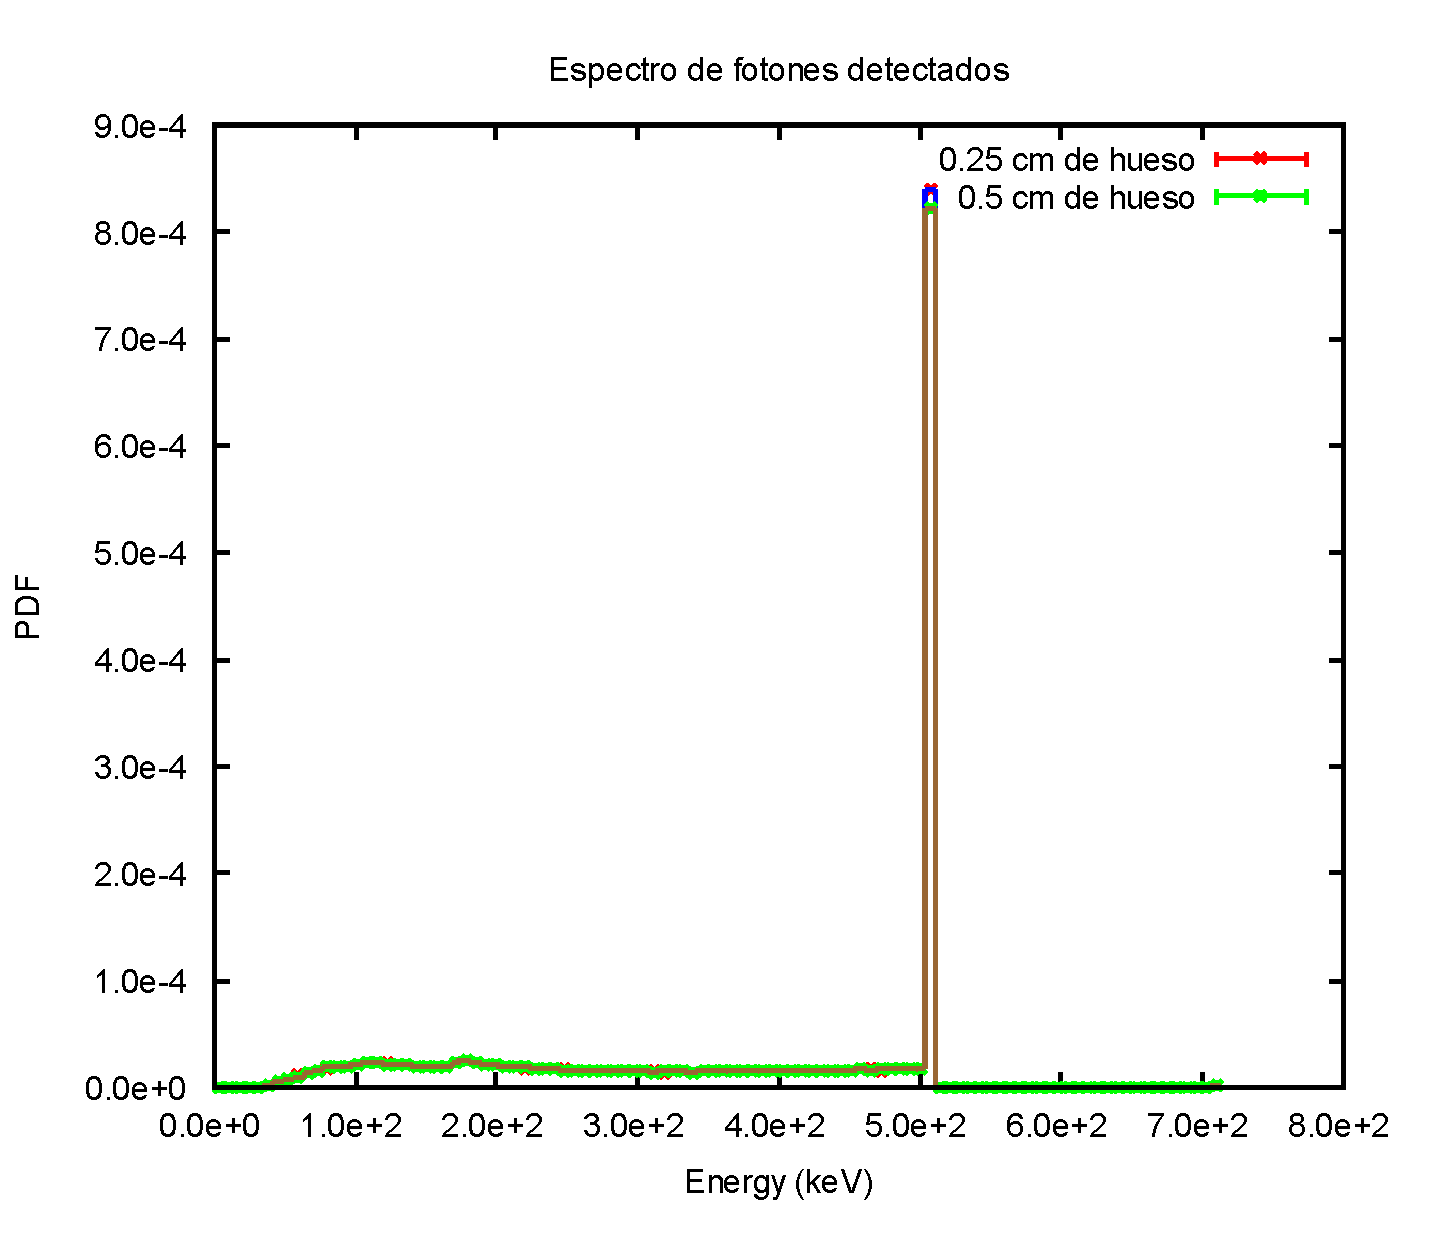
\includegraphics[scale=0.32]{025_05hueso}
		\caption{Espectro de energía de $\gamma$ usando \ce{^{18}F} en cabeza de 9 cm de radio con 0.5 cm y 0.25 cm de hueso.} 
		\label{fig:02505hueso}
	\end{minipage}
	\hspace{2mm}
	\begin{minipage}{0.45\textwidth}
		\centering
		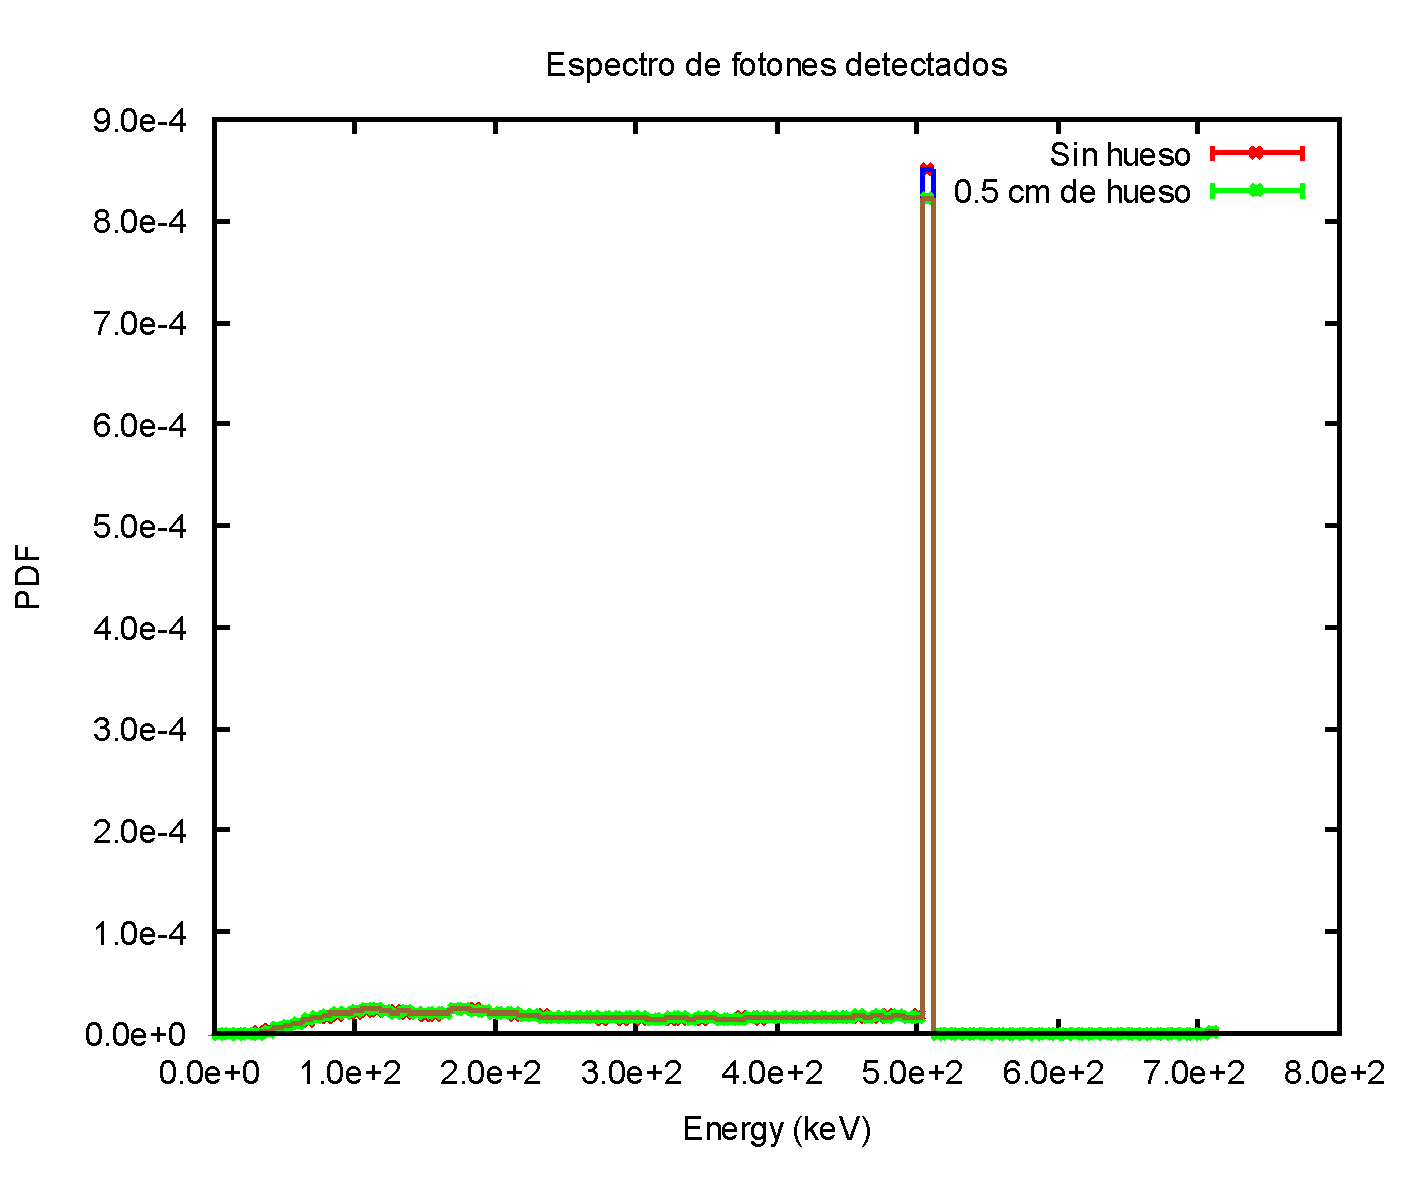
\includegraphics[scale=0.32]{2sinhueso05cmhueso}
		\caption{Espectro de energía de $\gamma$ usando \ce{^{18}F} en cabeza de 9 cm de radio con 0.5 cm de hueso, y sin hueso}
		\label{fig:2sinhueso05cmhueso}  
\end{minipage}	
\end{figure}
\begin{figure}[H]
	\centering
	\begin{minipage}{0.45\textwidth}
		\centering
		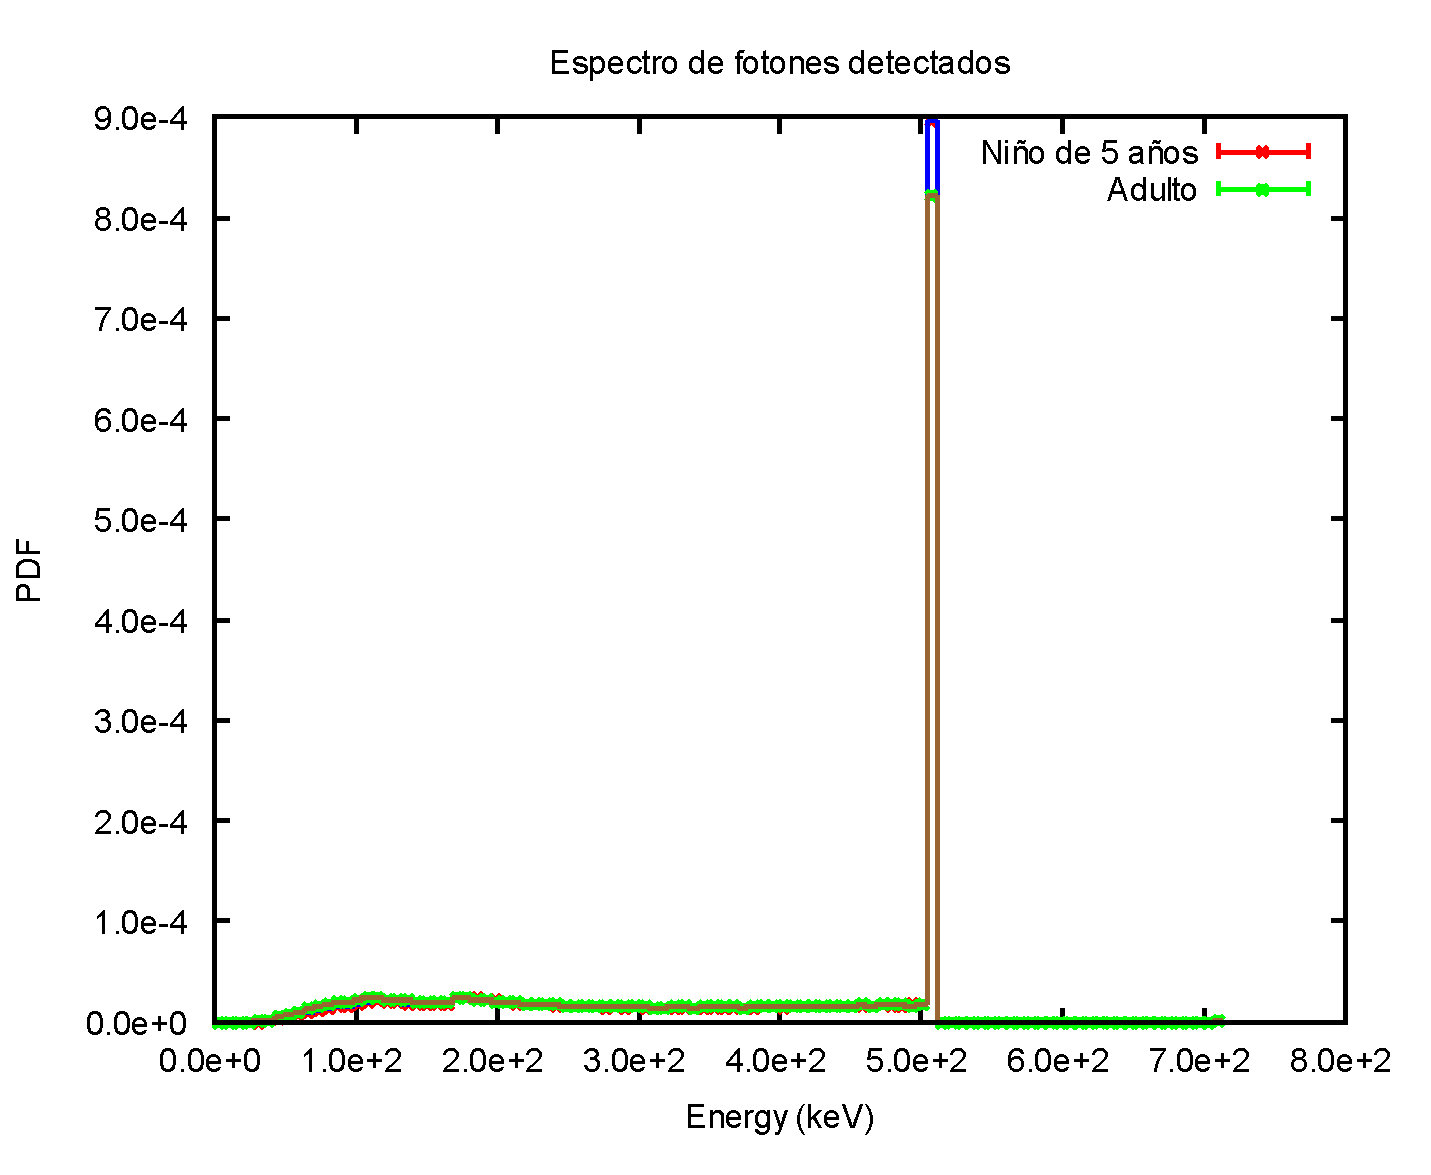
\includegraphics[scale=0.32]{2_nino5_vs_adulto}
		\caption{Espectro de energía de $\gamma$ usando \ce{^{18}F} en cabeza de un niño de 5 años (r = 8 cm) y un adulto (r = 9 cm), ambos con 0.5 cm de hueso.} 
		\label{fig:2nino5vsadult}
	\end{minipage}
	\hspace{2mm}
	\begin{minipage}{0.45\textwidth}
		\centering
		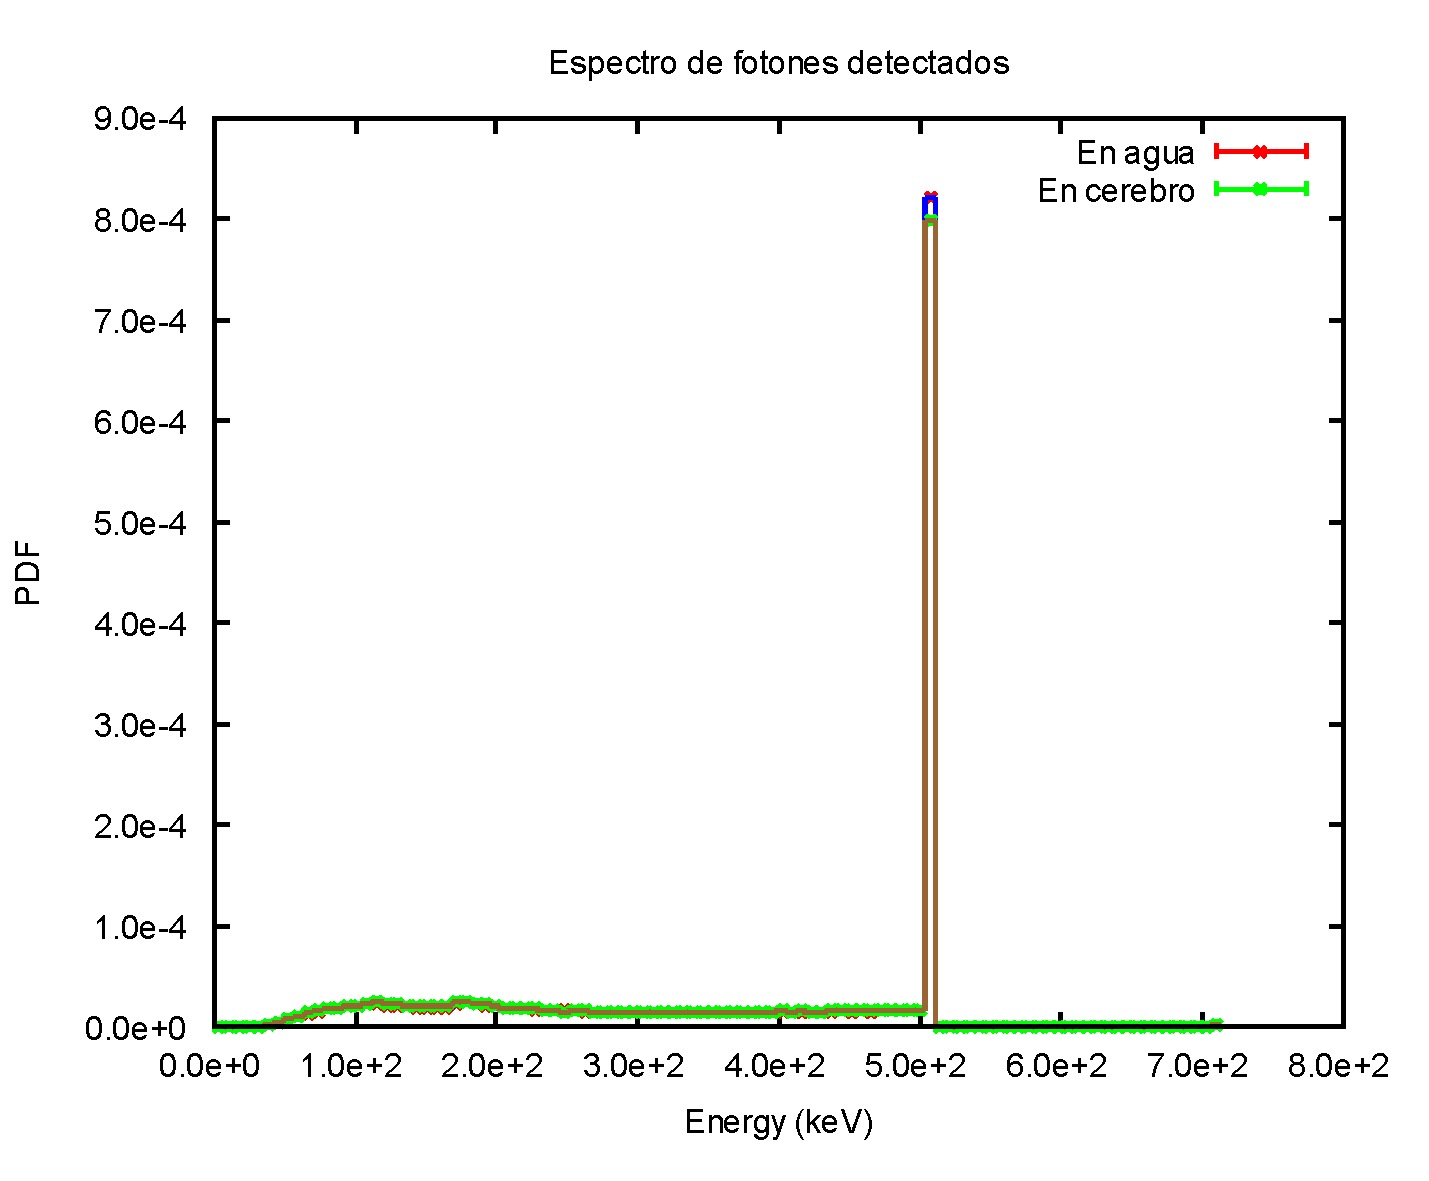
\includegraphics[scale=0.32]{2brainvswater}
		\caption{Espectro de energía de $\gamma$ usando \ce{^{18}F} en agua y cerebro con 0.5 cm de hueso y cabeza de 9 cm de radio.}
		\label{fig:2brainvswater}  
	\end{minipage}	
\end{figure}


En la figura \ref{fig:2nino5vsadult} se consideró el radio de la cabeza de un niño de 5 años con radio igual a 8 cm aproximadamente para analizar el espectro de los fotones detectados conjuntamente con el radio de la cabeza de un adulto igual a 9 cm, en ambos casos con 0.5 cm de hueso. Se observa que en el caso del niño es detectado un mayor número de fotones, pues el máximo de la PDF entre los dos casos es para el niño debido a que los fotones interactúan una menor distancia con el agua, pues el radio de su cabeza es 8 cm. Finalmente, en la figura \ref{fig:2brainvswater} se considera la misma geometría de la cabeza del adulto pero usando agua y cerebro, siendo ligeramente mayor el máximo de la PDF para el agua en comparación al cerebro, lo que significa que en el cerebro hay una mayor atenuación de los fotones.


\section{Conclusiones}
En PET-1 el espectro energético y la distribución de posiciones de aniquilación de los positrones varía de acuerdo a la energía máxima y alcance de cada radionúclido. En el primer caso se visualiza un espectro energético continuo, mientras que al usar una fuente monoenergética únicamente se visualiza un pico. Realizadas las simulaciones para cada radionúclido se observa que la distribución de posiciones de aniquilación usando la fuente monoenergética se muestra desplazada hacia la izquierda en contraste a cuando se considera el espectro continuo.

En el PET-2 se observó en primera instancia un máximo de la PDF para el \ce{^{18}F} en comparación a los otros radioisótopos, es decir que un mayor número de fotones llegan al detector usando este tipo de radioisótopo. Tras realizar algunas simulaciones reduciendo la corona esférica hasta desaparecerla se evidenció que aumenta el número de fotones en el detector debido a una menor atenuación, presentando una relación inversamente proporcional. Así mismo la atenuación presentada en cerebro es ligeramente mayor que en agua.

\bibliography{References}
\bibliographystyle{ieeetr}

\end{document}